%%%%%%%%%%%%%%%%%%%%%%%%%%%%%%%%%%%%%%%%%%%%%%%%%%%%%%%%%%%%%%%%%%%%%%%%%%%%%%%%%%
\begin{frame}[fragile]\frametitle{}
\begin{center}
{\Large Introduction to LangChain}
\end{center}
\end{frame}

%%%%%%%%%%%%%%%%%%%%%%%%%%%%%%%%%%%%%%%%%%%%%%%%%%%%%%%%%%%%%%%%%%%%%%%%%%%%%%%%%%
\begin{frame}\frametitle{What is LangChain?}

\begin{itemize}
\item Langchain is an open source framework for developing apps powered by language models
\item It is designed based on following principles:
	\begin{itemize}
	\item Be Data Aware: connect a language model to other sources of data
	\item Be Agentic: allow a language model to interact with its environment
	\end{itemize}
\item Currently it is available as python and javascript libraries
\item A project initiated by Harrison Chase, but now has rapidly growing contributor and user base (16.1k stars, 367 contributors, 2k forks \& used by 1.6k as of writing this post)!
\end{itemize}

{\tiny (Ref: Linkedin Post by Munjal Patel)}
\end{frame}

%%%%%%%%%%%%%%%%%%%%%%%%%%%%%%%%%%%%%%%%%%%%%%%%%%%%%%%%%%%%%%%%%%%%%%%%%%%%%%%%%%
\begin{frame}\frametitle{What is LangChain?}

\begin{itemize}
\item LangChain can be used to work with Large Language Models (LLMs). 
\item To answer questions about a specific field, like medicine or law. 
\item Popular framework for fine tuning with custom corpus.
\end{itemize}

\begin{center}
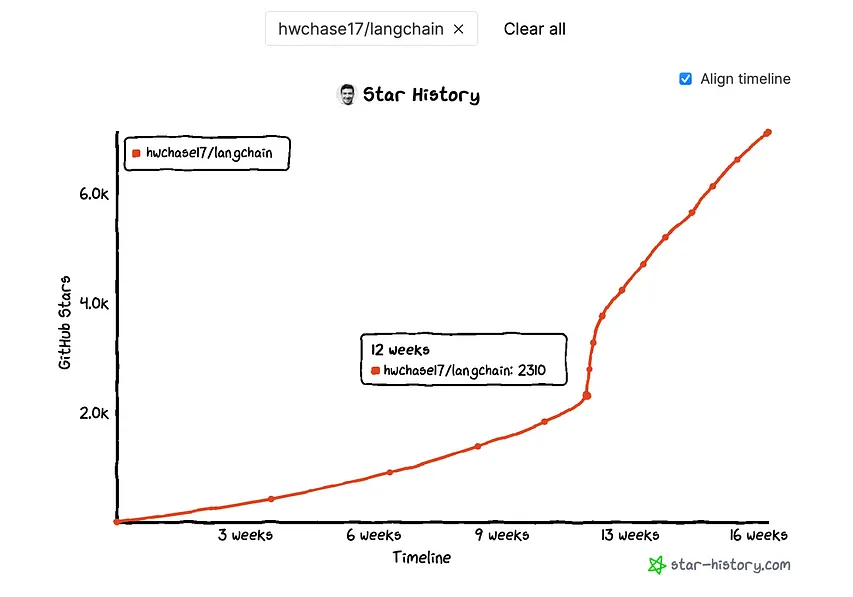
\includegraphics[width=0.6\linewidth,keepaspectratio]{langchain3}
\end{center}	  


{\tiny (Ref: Getting started with LangChain - Avra)}
\end{frame}

%%%%%%%%%%%%%%%%%%%%%%%%%%%%%%%%%%%%%%%%%%%%%%%%%%%%%%%%%%%%%%%%%%%%%%%%%%%%%%%%%%
\begin{frame}\frametitle{Why LangChain?}

\begin{itemize}
\item LLMs and Prompts: Prompt management, Prompt optimization, Generic interface for all LLMs and Common utilities for working with LLMs
\item Chains: Chains are sequences of calls that whether to an LLM or a different utility. LangChain provides a standard interface for chains, many integrations with other tools, \& end-to-end chains for common applications.
\item Extenal Data Augmentation: Specific types of chains that first interact with an external data source to fetch data to use in the generation step. Examples of this include summarization of long pieces of text \& question/answering over specific data sources
\item Agents: Agents involve an LLM making decisions about which actions to take, taking that action, seeing an observation, \& repeating that until done. LangChain provides a standard interface for agents, a selection of agents to choose from, and examples of end-to-end agents.
\item Memory: Memory refers to the concept of persisting state between calls of a chain/agent. LangChain provides a standard interface for memory, a collection of memory implementations, and examples of chains/agents that use memory.
\item Evaluation [BETA]: Generative models are notoriously hard to evaluate with traditional metrics. One new way of evaluating them is using language models themselves to do the evaluation. LangChain provides some prompts/chains for assisting in this.
\end{itemize}

{\tiny (Ref: Linkedin Post by Munjal Patel)}
\end{frame}

%%%%%%%%%%%%%%%%%%%%%%%%%%%%%%%%%%%%%%%%%%%%%%%%%%%%%%%%%%%%%%%%%%%%%%%%%%%%%%%%%%
\begin{frame}\frametitle{LangChain Usecases}

\begin{itemize}
\item Personal assistants
\item Question answering over database(s)
\item Chatbots
\item Querying tabular data
\item Interacting with APIs
\item Model Evaluation
\end{itemize}


{\tiny (Ref: Linkedin Post by Munjal Patel)}
\end{frame}


%%%%%%%%%%%%%%%%%%%%%%%%%%%%%%%%%%%%%%%%%%%%%%%%%%%%%%%%%%%%%%%%%%%%%%%%%%%%%%%%%%
\begin{frame}\frametitle{How LangChain Works?}

\begin{itemize}
\item Text is preprocessed by breaking it down into chunks or summaries, 
\item embedding them in a vector space, 
\item searching for similar chunks when a question is asked. 
\end{itemize}

\begin{center}
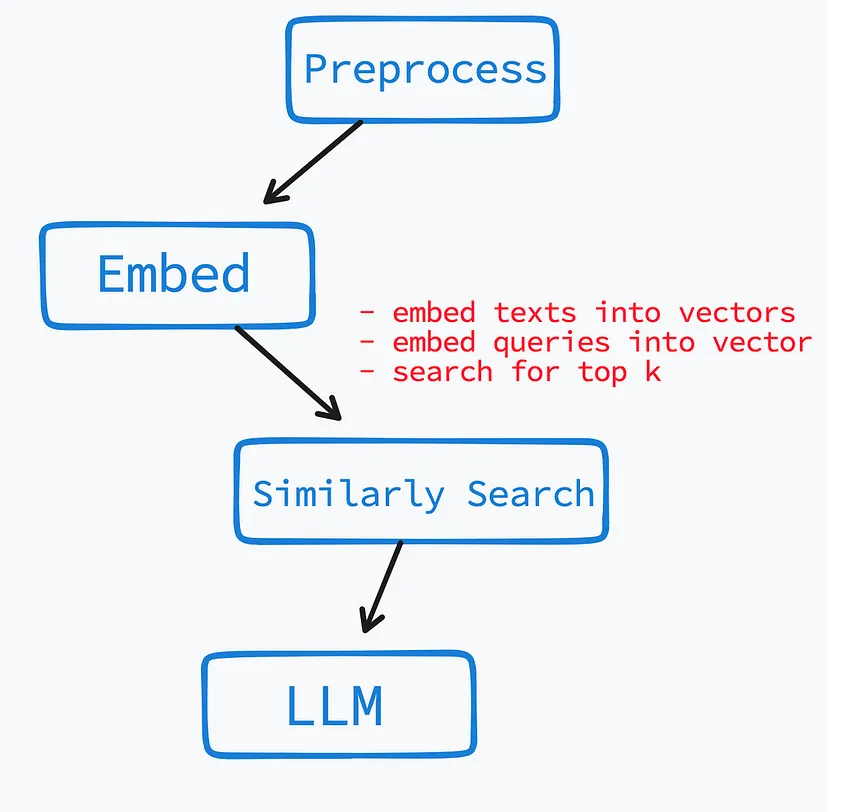
\includegraphics[width=0.5\linewidth,keepaspectratio]{langchain4}
\end{center}	  


{\tiny (Ref: Getting started with LangChain - Avra)}
\end{frame}


%%%%%%%%%%%%%%%%%%%%%%%%%%%%%%%%%%%%%%%%%%%%%%%%%%%%%%%%%%%%%%%%%%%%%%%%%%%%%%%%%%
\begin{frame}\frametitle{LangChain Components}

\begin{center}
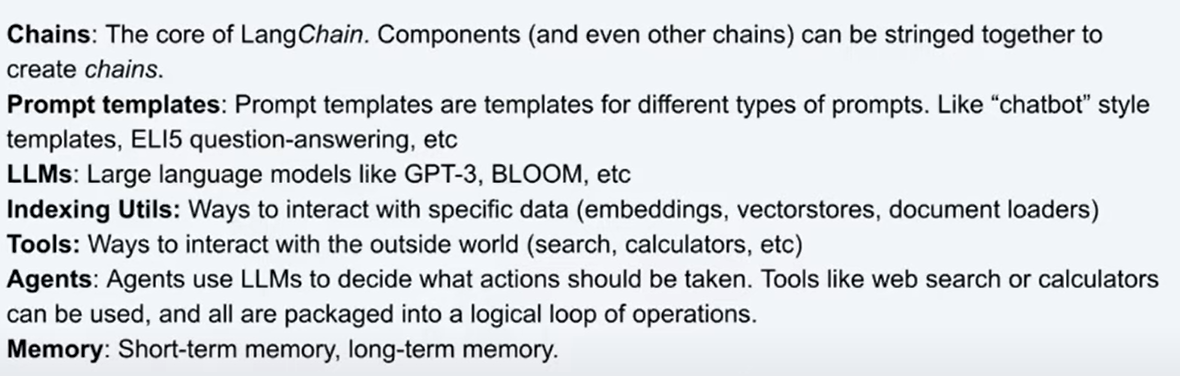
\includegraphics[width=\linewidth,keepaspectratio]{langchain1}
\end{center}	  

{\tiny (Ref: Building the Future with LLMs, LangChain, \& Pinecone)}
\end{frame}

%%%%%%%%%%%%%%%%%%%%%%%%%%%%%%%%%%%%%%%%%%%%%%%%%%%%%%%%%%%%%%%%%%%%%%%%%%%%%%%%%%
\begin{frame}\frametitle{Chains}

\begin{itemize}
\item Enable users to combine multiple components together to create a single, coherent application.
\item Example: takes user input, formats it using a PromptTemplate, and then passes the formatted response to a Large Language Model (LLM) for processing.
\item Sequential chains: output of the first LLM becomes the input to the second LLM and so on
\end{itemize}

\begin{center}
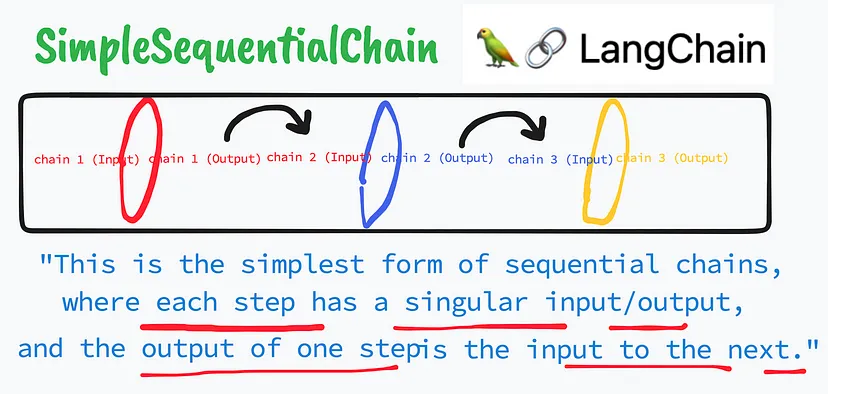
\includegraphics[width=0.8\linewidth,keepaspectratio]{langchain5}
\end{center}	  


{\tiny (Ref: Getting started with LangChain - Avra)}
\end{frame}

%%%%%%%%%%%%%%%%%%%%%%%%%%%%%%%%%%%%%%%%%%%%%%%%%%%%%%%%%%%%%%%%%%%%%%%%%%%%%%%%%%
\begin{frame}[fragile] \frametitle{Chains}

{\tiny (Ref: Getting started with LangChain - Avra)}


\begin{lstlisting}
    # Chain 1: Generating a rephrased version of the user's question
    template = """{question}\n\n"""
    prompt_template = PromptTemplate(input_variables=["question"], template=template)
    question_chain = LLMChain(llm=llm, prompt=prompt_template)

    # Chain 2: Generating assumptions made in the statement
    template = """Here is a statement:
        {statement}
        Make a bullet point list of the assumptions you made when producing the above statement.\n\n"""
    prompt_template = PromptTemplate(input_variables=["statement"], template=template)
    assumptions_chain = LLMChain(llm=llm, prompt=prompt_template)
    assumptions_chain_seq = SimpleSequentialChain(
        chains=[question_chain, assumptions_chain], verbose=True
    )

\end{lstlisting}

\end{frame}

%%%%%%%%%%%%%%%%%%%%%%%%%%%%%%%%%%%%%%%%%%%%%%%%%%%%%%%%%%%%%%%%%%%%%%%%%%%%%%%%%%
\begin{frame}[fragile] \frametitle{Chains}

{\tiny (Ref: Getting started with LangChain - Avra)}


\begin{lstlisting}
    # Chain 3: Fact checking the assumptions
    template = """Here is a bullet point list of assertions:
    {assertions}
    For each assertion, determine whether it is true or false. If it is false, explain why.\n\n"""
    prompt_template = PromptTemplate(input_variables=["assertions"], template=template)
    fact_checker_chain = LLMChain(llm=llm, prompt=prompt_template)
    fact_checker_chain_seq = SimpleSequentialChain(
        chains=[question_chain, assumptions_chain, fact_checker_chain], verbose=True)
    # Final Chain: Generating the final answer to the user's question based on the facts and assumptions
    template = """In light of the above facts, how would you answer the question '{}'""".format(user_question)
    template = """{facts}\n""" + template
    prompt_template = PromptTemplate(input_variables=["facts"], template=template)
    answer_chain = LLMChain(llm=llm, prompt=prompt_template)
    overall_chain = SimpleSequentialChain(
        chains=[question_chain, assumptions_chain, fact_checker_chain, answer_chain],
        verbose=True,)
\end{lstlisting}


\end{frame}

%%%%%%%%%%%%%%%%%%%%%%%%%%%%%%%%%%%%%%%%%%%%%%%%%%%%%%%%%%%%%%%%%%%%%%%%%%%%%%%%%%
\begin{frame}\frametitle{Chains}

The SimpleSequentialChain combines several chains of operations to run a pipeline. 

\begin{itemize}
\item question\_chain: This chain takes the user's question as input and returns it as output. 
\item assumptions\_chain: This chain takes the output from question\_chain as input and produces a bullet-point list of assumptions based on a statement related to the question. 
\item fact\_checker\_chain: This chain takes the outputs from question\_chain and assumptions\_chain as inputs and produces a bullet-point list of assertions based on the question and assumptions.
\item answer\_chain: This chain takes the outputs from question\_chain, assumptions\_chain, and fact\_checker\_chain as inputs and produces an answer to the user's question based on the facts generated by the previous chains.
\end{itemize}


{\tiny (Ref: Getting started with LangChain - Avra)}
\end{frame}


%%%%%%%%%%%%%%%%%%%%%%%%%%%%%%%%%%%%%%%%%%%%%%%%%%%%%%%%%%%%%%%%%%%%%%%%%%%%%%%%%%
\begin{frame}\frametitle{Prompt Engineering}

\begin{center}
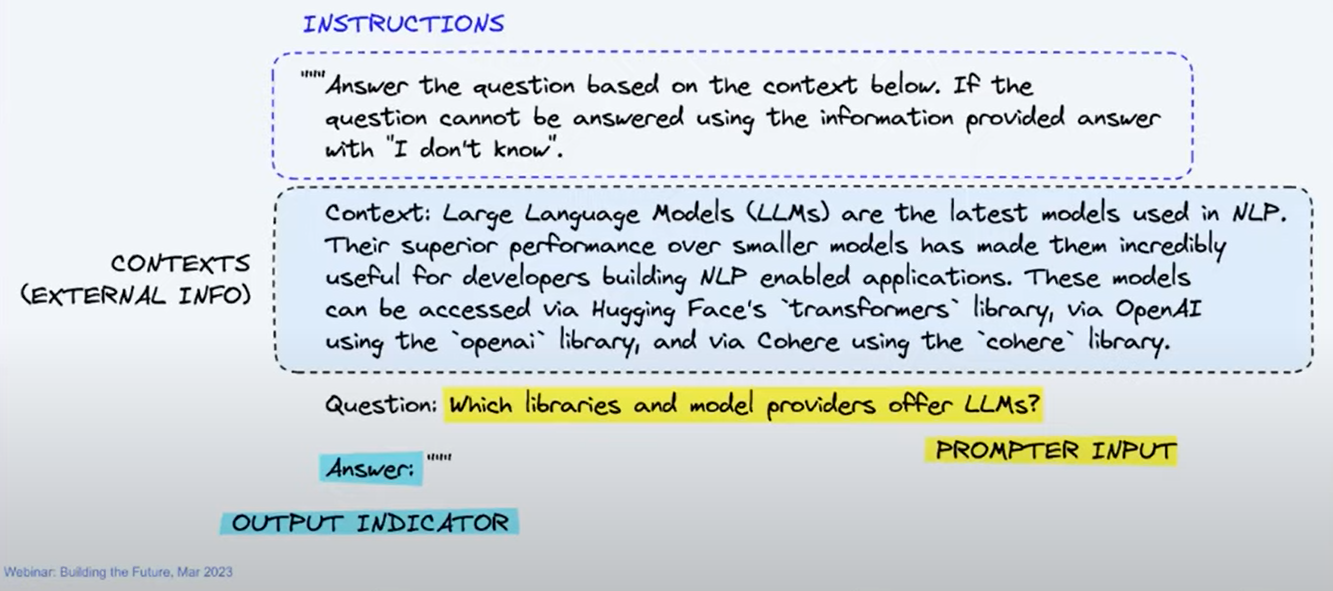
\includegraphics[width=\linewidth,keepaspectratio]{langchain2}
\end{center}	  

{\tiny (Ref: Building the Future with LLMs, LangChain, \& Pinecone)}
\end{frame}

%%%%%%%%%%%%%%%%%%%%%%%%%%%%%%%%%%%%%%%%%%%%%%%%%%%%%%%%%%%%%%%%%%%%%%%%%%%%%%%%%%
\begin{frame}\frametitle{References}


\begin{itemize}
\item Official doc: https://docs.langchain.com/docs/
\item Git Repo: https://github.com/hwchase17/langchain
\item Cookbook by Gregory Kamradt(Easy way to get started): https://github.com/gkamradt/langchain-tutorials/blob/main/LangChain\%20Cookbook.ipynb
\item Youtube Tutorials: https://www.youtube.com/watch?v=\_v\_fgW2SkkQ\&list=PLqZXAkvF1bPNQER9mLmDbntNfSpzdDIU5
\end{itemize}


\end{frame}